% Chapter Template

\chapter{Chromospheric emission - age relationship} % Main chapter title

\label{Chapter4} % Change X to a consecutive number; for referencing this chapter elsewhere, use \ref{ChapterX}

\epigraph{\itshape There is a way out of every box, a solution to every puzzle; it's just a matter of finding it.}{---Captain Jean-Luc Picard, \itshape Star Trek}

\section{Introduction}
\textcolor{red}{RB: If this paper is published before submitting - put paragraph similar to the one in Chapter 3 here!}

In \citet{Booth_etal_2017} a steepening of the age-activity relationship was found using X-ray observations coupled to asteroseismic ages. While this study provided the first step to studying the X-ray luminosity-age relationship beyond a gigayear, using the X-ray luminosity as a magnetic activity indicator may not be the most accessible indicator as it requires significant observational resources on an X-ray telescope. An alternative magnetic activity indicator is chromospheric emission in spectral lines such as \caII or H$-\alpha$. Particularly for exoplanet host stars, optical spectra are usually obtained to confirm the presence of candidate exoplanets through radial velocity measurements; therefore making chromospheric emission a much more commonly used magnetic activity indicator.

Chromospheric emission is a widely used activity indicator, particularly for the age-activity relationship and there have been several studies in recent years that use this indicator to calibrate the relationship. However, some debate remains over the suitability of chromospheric emission seen in \caII lines as an age indicator for older stars (i.e. $> 1$ Gyr). \citet{Pace_2013} shows an L-shaped age-activity plot and suggested that the evolution of the chromospheric emission in the \caII lines stopped relatively early. On the contrary, \citet{Lorenzo_Oliveira_etal_2016} showed that when the mass and metallicity of the star is taken into account, chromospheric ages show good agreement with asteroseismic ages. Yet, both of these studies use isochronal ages to calibrate their relationships, asteroseismic ages have not been studied in relation to the chromospheric emission - age relationship. Therefore, the aim of this work was to investigate the age-activity relationship beyond a gigayear using chromospheric emission as a magnetic activity indicator coupled with asteroseismic ages to help shed light on its suitability as an age indicator.

\textcolor{red}{Insert description of each section - so that I can explain that most of the work is focused on Ca but did some analysis on H-alpha}

\section{Observations}
\subsection{Sample selection}
The sample considered in this work were selected from stars studied by \citet{Bruntt_etal_2012}, who performed a detailed spectral study aided by asteroseismic data for 93 solar-type stars observed with \textit{Kepler}. For the purposes of studying the magnetic activity of old stars, the sample was restricted to stars with an outer convective envelope, are on the main sequence and have an asteroseismically determined age.

In order to select stars with an outer convective envelope, the effective temperature was required to be less than 6500 K, equivalent to spectral type F5V. Stars with spectral types earlier than F5V do not have a substantial outer convective envelope that is required for the solar-like dynamo process \citep{Pinsonneault_etal_2001}. Therefore, these stars are not expected to spin-down via magnetic braking during their main sequence lifetime or follow the same age-activity relationship as lower-mass stars. However, there is some observational evidence that hotter stars can occasionally display magnetic activity features as well; for example, weak X-ray emission was detected from the A7V star Altair \citep{Robrade_Schmitt_2009}. Therefore, data analysis was performed on all main sequence stars in the sample spanning the full effective temperature range of ca. 5000-6900 K, but stars with effective temperatures greater than 6500 K are displayed separately in tables and figures.

Stars that have significantly evolved off the main sequence are expected to have different rotational and magnetic evolution, therefore only stars that are still on the main sequence should be included in the age-activity analysis. To ensure that the stars in the sample were on the main sequence, their surface gravities \citep{Bruntt_etal_2012} from asteroseismology (\textcolor{red}{Triple check I used the Brunnt log(g) asteroseismic values} to the relation between $B-V$ colour and surface gravity for main sequence stars as given by \citet{Gray_2005} and shown in Equation \ref{Eq:Gray_2005}. Stars with surface gravities that differed by more than 0.2 dex were excluded from the sample.

Stellar ages from asteroseismology were collected from the literature. In particular, ages from \citet{Silva_Aguirre_etal_2017} were used for the majority of the sample, where stellar ages were obtained by modelling the individual oscillation frequencies in the spectrum observed by the \textit{Kepler} satellite. Some ages were also taken from \citet{Chaplin_etal_2014}, where stellar properties were estimated using two global asteroseismic parameters and complementary photometric and spectroscopic data.

\subsection{Spectra}
The spectra used in this study stem from \citet{Bruntt_etal_2012}. The spectra were obtained with the \esp spectrograph at the 3.6 m Canada-France-Hawaii Telescope (CFHT; \citealt{Donati_etal_2006}) and the \narval spectrograph \citep{Auriere_2003} mounted on the 2 m Bernard Lyot Telescope at the Pic du Midi Observatory. These spectra cover a spectral range of ${\thicksim} 3700$ to ${\thicksim} 10480$ \AA. In this work, the reduced spectra by \citet{Bruntt_etal_2012} was used which was received through personal communication. In \citet{Bruntt_etal_2012}, standard pipeline-reduced spectra were normalised using \texttt{RAINBOW} \citep{Bruntt_etal_2010} which allows manual normalisation of the spectra. The continua were adjusted by comparing with a synthetic spectrum and overlapping regions of spectral orders were checked so that both the line depths and continuum level matched.

Additional archival observations were used to investigate the level of long-term variability of the \Rprime indicator due to potential magnetic activity cycles (see Section REF). Pipeline-reduced spectra were obtained directly from the \esp archive\footnote{\url{http://www.cadc-ccda.hia-iha.nrc-cnrc.gc.ca/en/}}.

In the following sections (i.e Sections \ref{Chp4_data_analysis}, \ref{Chp4_results} and \ref{Chp4_discussion}), the focus will be on the data analysis, results and discussion of the chromospheric emission from the \caII spectral lines.

\section{Data Analysis}
\label{Chp4_data_analysis}

In this section, the process to extract the chromospheric emission from the \caII lines is described. It details the processing of the spectra data, the calibration of the emission to the Mount Wilson S index and how the final \Rprime indicator value was calculated. Section \ref{Chp4_halpha} will discuss the analysis performed on the H-$\alpha$ spectral line.

\subsection{Doppler correction}
\label{Chp4_data_analysis_doppler}
The first step in the data analysis was to correct for any Doppler shift present in the stellar spectrum. Doppler shifts in spectra are a common occurrence in astronomical spectra due to the relative motions of stars and is seen as a change in the wavelength that spectral lines are observed at. Since the relative motions of each of the stars is slightly different, then the core of the \caII lines (where the chromospheric emission is observed) will be observed at slightly different wavelengths. In order to analyse the correct part of the spectral lines the Doppler shift must be accounted for; this is achieved by comparing all spectra to one master spectrum and adjusting the wavelength scale so that spectral line coincide at the same wavelength.

A master spectrum was selected by considering the signal to noise ratio (hereafter SNR) in the 3850 to 4050 \AA wavelength region. The SNR was calculated using Equation \ref{Eq:SNR_ratio} where $\bar{f}$ is the mean flux value and $\sigma_{f}$ is the standard deviation of the flux in the relevant wavelength region. The spectrum with the largest SNR value was chosen as the master spectrum to which all other spectra were compared to; the master spectra were KIC 9226926 and KIC 3733735 for the \narval and \esp spectra, respectively.

\begin{equation}
SNR = \frac{\bar{f}}{\sigma_{f}}
\label{Eq:SNR_ratio}
\end{equation}

A cross correlation function was then used to compare each of the spectra to the master spectrum; this function measures the similarity of a spectrum to the master spectrum as a function of the relative displacement. The maximum of the cross correlation function was then used to determine the relative displacement that must be taken into account for the two spectra to be aligned. The relative displacement was applied to the spectrum, allowing analysis of the \caII lines using the same wavelength regions for all spectra. An additional manual wavelength correction was applied to the spectra in order to to compensate for any Doppler shift that was present in the master spectrum. This was $-0.2$ \space \AA for the \esp data; the \narval data did not require this manual correction.

\subsection{Normalisation of continuum}
\label{Chp4_data_analysis_normalise_cont}
Before the \Rprime indicator could be calculated, the spectra were required to be normalised as there was a discontinuity in the continuum at the \caII wavelengths. This is shown in the top panel of Figure \ref{fig:normlisation_example}; the flux in the overlapping region match reasonably well, but the continuum level flux level is higher in the K order than the H order. This would have an effect on the chromospheric emission measurement as the method used (see Section \ref{Chp4_data_analysis_calc_S}) requires the flux measured in the core of the \caII lines to be normalised by the flux continuum in two reference channels.

\begin{figure}
    \centering
    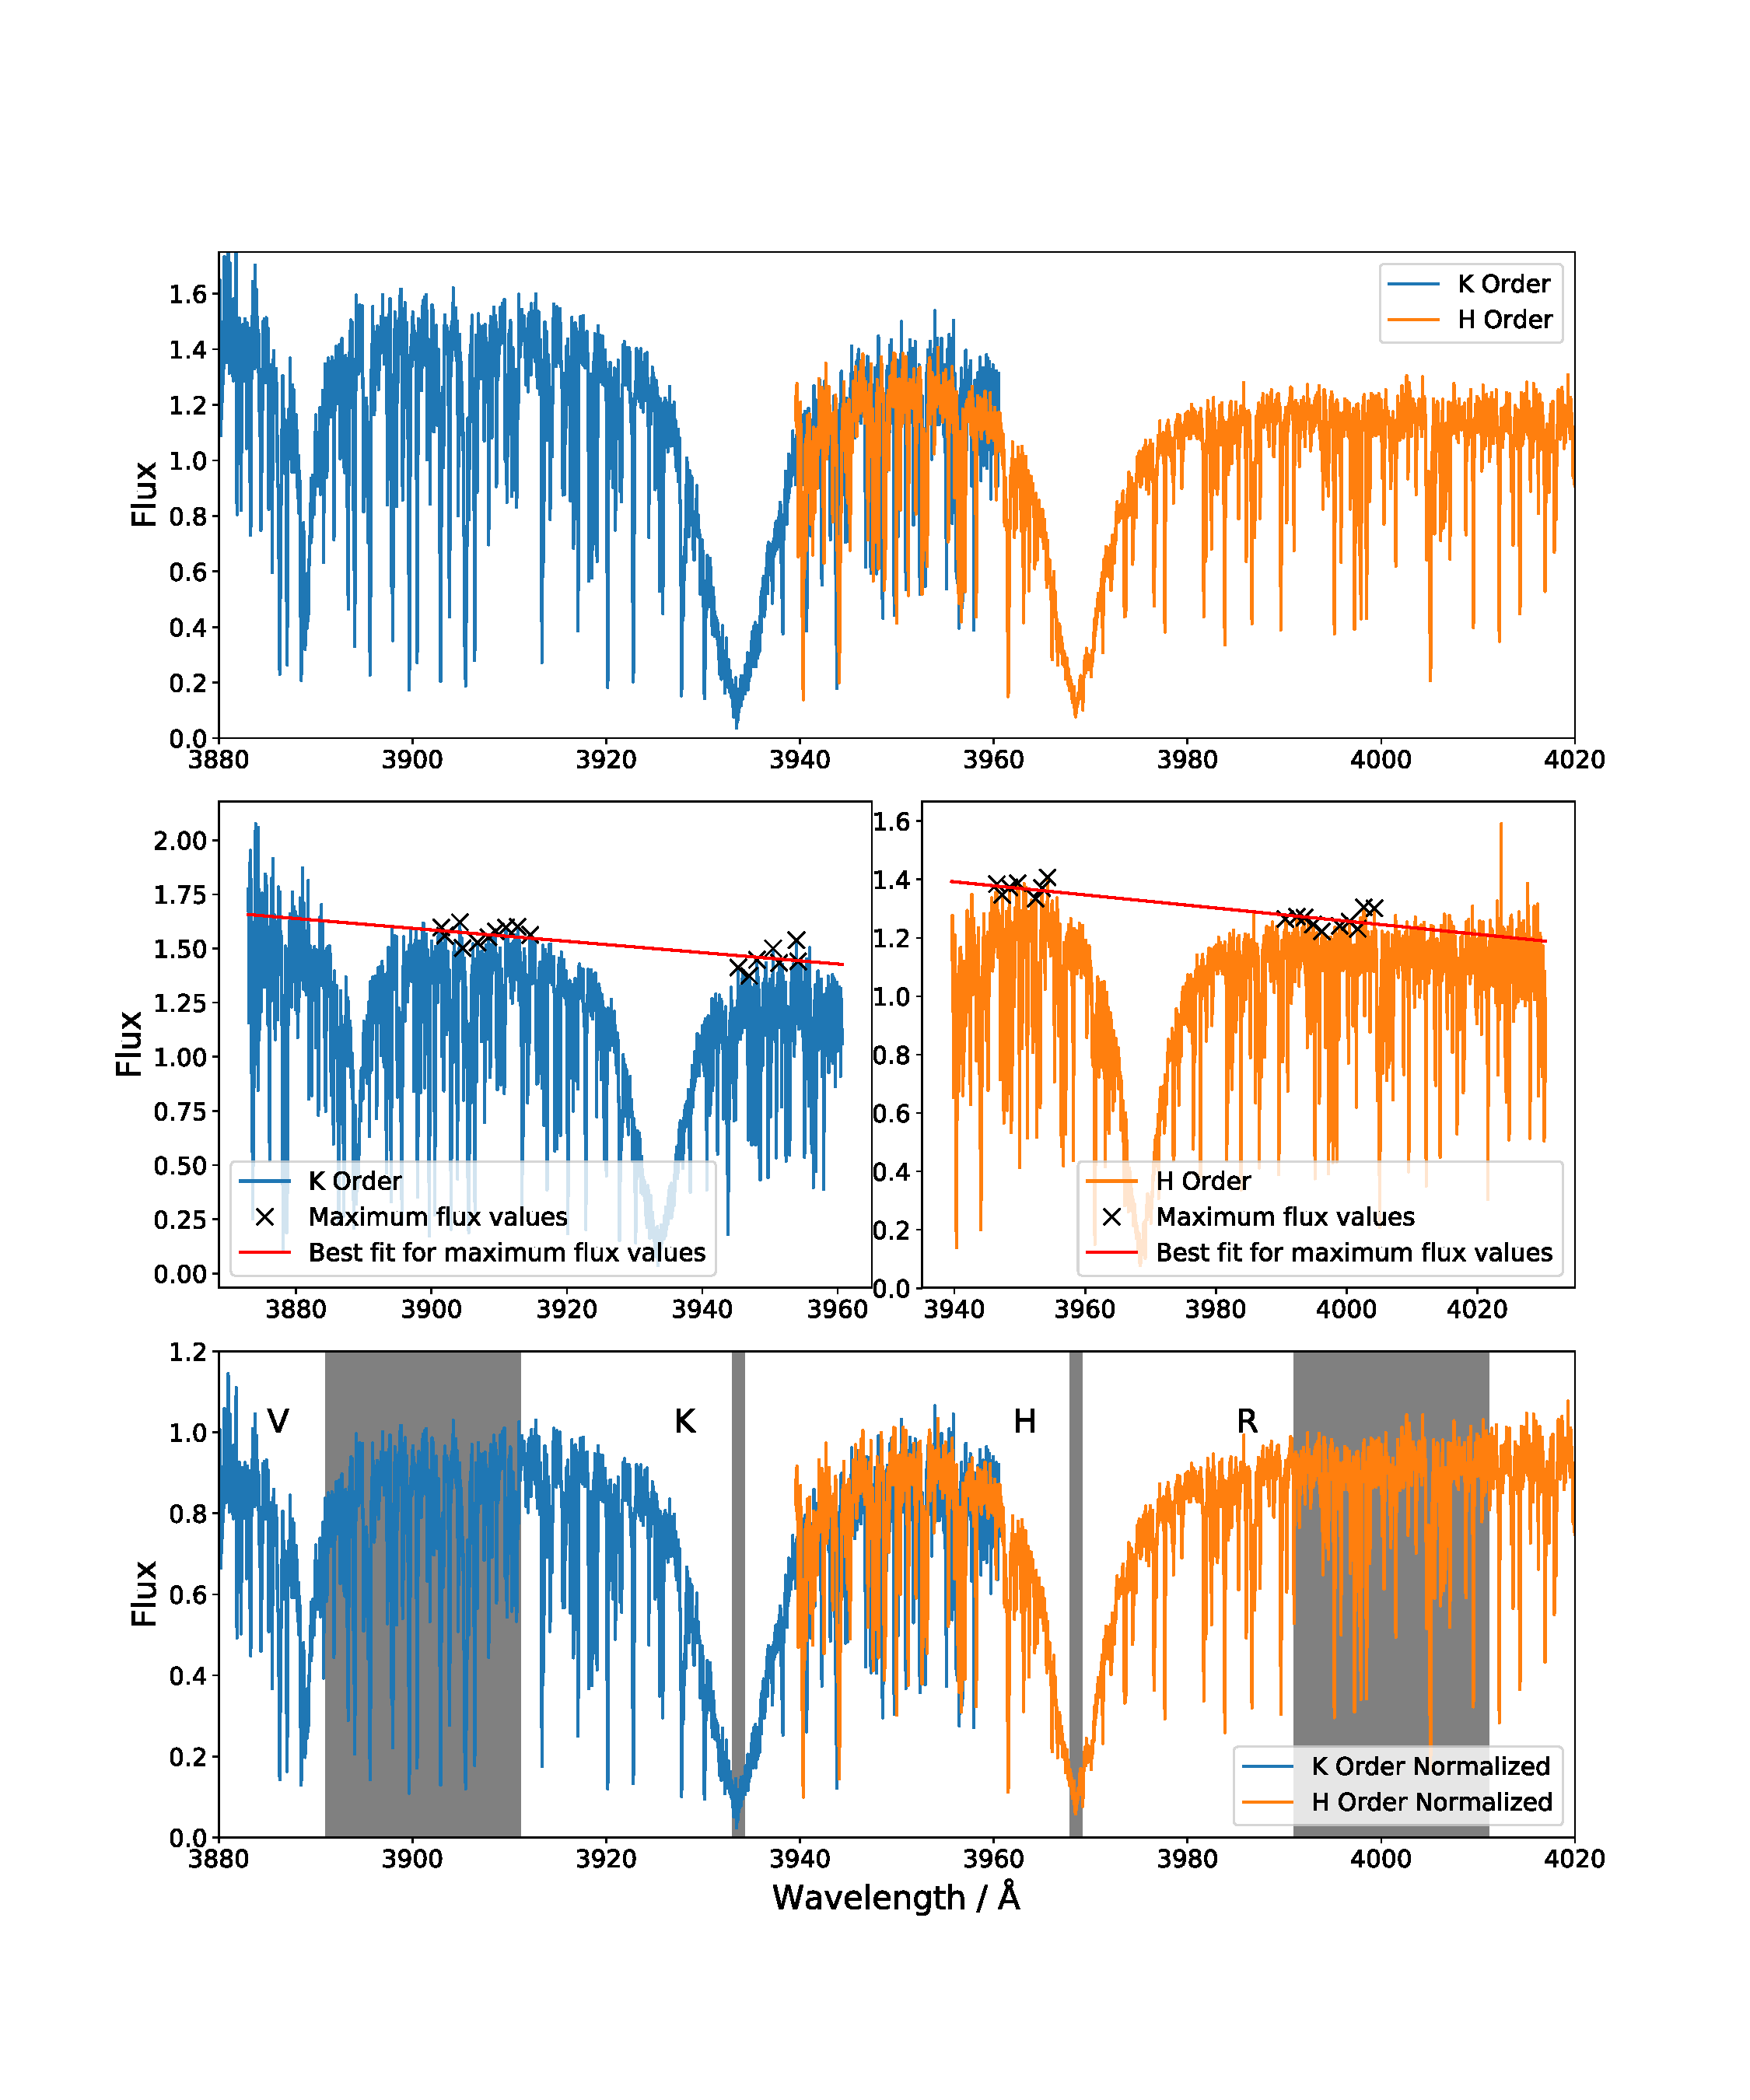
\includegraphics[scale=0.40]{Figures/4-Chromospheric_age/kic9139163_example.pdf}
    \caption[Example of optical spectra in \caII region and the normalisation method]{\textbf{Top panel:} Spectrum of KIC 9139163 showing the two adjacent spectral orders that contain the \caII lines. While the overlapping region of the orders match, there is a clear discontinuity in the continuum flux level.
    \textbf{Middle panel:} Plots of the two comparison regions in the K order (left) and H order (right). The markers denote the maximum flux values in each bin of width 1.5 \AA. The red line denotes the best-fitting linear relationship that is used to normalise the spectrum.
    \textbf{Bottom panel:} Spectrum of KIC 9139163 with correction factor applied to the K order. The discontinuity in the continuum flux level is no longer present. The four channels used to calculate the S index are also shown.}
    \label{fig:normlisation_example}
\end{figure}

This was corrected by considering two comparison regions in each spectral order; from 3900 - 3915 \AA \space and 3945 - 3955 \AA \space in the shorter-wavelength order of the spectrum (containing the Ca~II K line) and from 3945 - 3955 \AA \space and 3990 - 4005 \AA \space in the longer-wavelength order of the spectrum (containing the Ca~II H line) as shown in the middle panel of Figure \ref{fig:normlisation_example}. The local continuum level was estimated in those regions by splitting the spectrum into bins of 1.5 \AA \space width and measuring the local maximum in each of the bins (see Figure \ref{fig:normlisation_example}). These data points were used to find the best-fitting linear relationship as indicated by the red line in the middle panel of Figure \ref{fig:normlisation_example}. The spectra were then normalised according to this best fitting relationship so that the typical continuum flux value in each order was approximately one.

\subsection{Calculation of S index}
\label{Chp4_data_analysis_calc_S}
The S index is an activity indicator that uses four channels to quantify the chromospheric emission in the core of the \caII lines. Two channels are 1.09 \AA \space wide and centred on 3968.47 and 3933.664 \AA \space for the \caII cores, respectively. The other two channels are 20 \AA \space wide and are centred on 3901.07 and 4001.07 \AA; named the V and R channels respectively. These channels are shown in the bottom panel of Figure \ref{fig:normlisation_example} and follow the channels defined by \citet{Lovis_etal_2011} with the exception that the triangular-shaped profile to the H and K channels are not included in this analysis.

The S index is calculated using Equation \ref{Eq:sindex} where $N_{x}$ is the total flux in the relevant channel. The error associated with $N_{x}$ is calculated using Equation \eqref{Eq:sindex_error} where $x_{n}$ is the error on the individual flux data point and $i$ is the total number of data points in the wavelength channel. These errors associated with $N_{x}$ were then propagated in order to calculate the error associated with the S index.

\begin{equation}
S = \frac{N_{H} + N_{K}}{N_{R} + N_{V}}
\label{Eq:sindex}
\end{equation}

\begin{equation}
\sigma_{N_{x}} = \sqrt{\sum_{n=1}^{i} x_{n}^{2}}
\label{Eq:sindex_error}
\end{equation}


\subsection{Calibration to \texorpdfstring{\Smw}{Smw} and calculating the \texorpdfstring{\Rprime}{Rprime} indicator}

\begin{figure}
    \centering
    \begin{subfigure}{\textwidth}
        \centering
        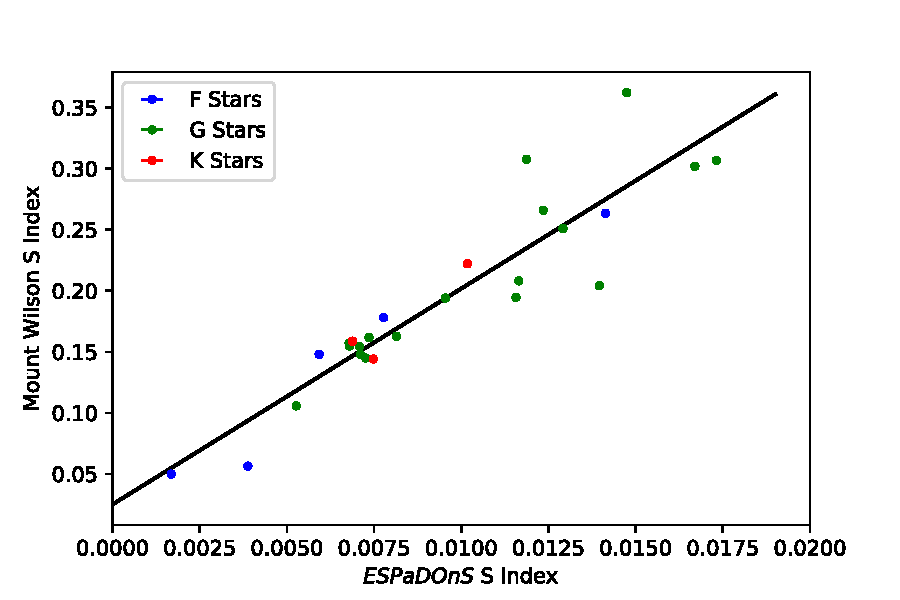
\includegraphics[scale=0.75]{Figures/4-Chromospheric_age/espadons_calibrator_reltionship.pdf}
        \caption{\esp Calibrators}
    \end{subfigure}
    \begin{subfigure}{\textwidth}
        \centering
        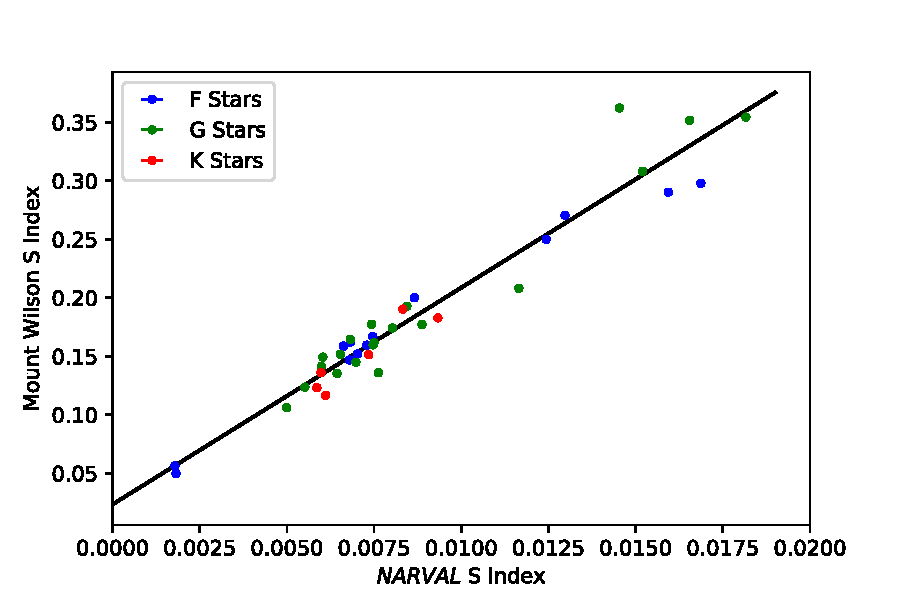
\includegraphics[scale=0.75]{Figures/4-Chromospheric_age/narval_calibrator_reltionship.pdf}
        \caption{\narval Calibrators}
    \end{subfigure}
    \caption{Plots showing the average \Smw \citep{Duncan_etal_1991} against the S index calculated from the \esp/\narval spectrographs for the calibrator stars. The black line indicates the best-fitting linear relationship between the two parameters.}
    \label{fig:calibrator_relationships_Smw}
\end{figure}

The method that is used to calculate the \Rprime indicator (\citealt{Noyes_etal_1984}; see Section \ref{chromospheric_emission_subsub}) requires the Mount Wilson S index (\Smw), which differs slightly from the S index calculated for the sample of stars considered in this work. The S index calculated in any spectrum (regardless of the exact method used) is dependent on the spectral resolution and the throughput of the spectrograph used. therefore it was necessary to determine a relationship between the S index calculated from the spectrographs used in this work (\esp and \narval) and \Smw. This was achieved by searching for stars from \citet{Duncan_etal_1991} in the \esp and \narval archives. \citet{Duncan_etal_1991} summarises measurements of \caII emission at the Mount Wilson Observatory from 1966 - 1983, thus providing a large sample of stars with measured \Smw values. The comparison sample was restricted to have the same range of spectral type as used in the analysis of old inactive stars, i.e. from spectral type F5 to late K. The stars from \citet{Duncan_etal_1991} with archival observations from \esp and \narval were Doppler corrected and normalised using the sample method as the main sample (see Section \ref{Chp4_data_analysis_doppler} and \ref{Chp4_data_analysis_normalise_cont}). The master spectra for Doppler correction were HD 89449 and HD 126660 for \esp and \narval data, respectively. The manual wavelength shift was -0.14 and +0.1 \AA \space for the \esp and \narval data, respectively. The full list of stars and values used to calibrate the two relationships are shown in Appendix \ref{App_calibrator_stars_Smw}.

The S index was calculated for these calibrator stars as described in Section \ref{Chp4_data_analysis_calc_S} and plotted against the mean \Smw from \citet{Duncan_etal_1991} (shown in Figure \ref{fig:calibrator_relationships_Smw}). Since the sample considered in this work contains weakly inactive stars older than a gigayear, we restricted the calibrator star sample to S index values less than 0.2 and \Smw values less than 0.5. A linear least-squares regression was applied to the data to find the best-fitting relationship between the two indices, which are shown in Equations \ref{Eq:esp_calibrator_eq} and \ref{Eq:nar_calibrator_eq}. These equations were used to calculate the \Smw for our sample of stars with asteroseismic ages.

\begin{equation}
S_{MW} = 17.67 \cdot S_{\mathrm{ESPaDOnS}}+ 0.025
\label{Eq:esp_calibrator_eq}
\end{equation}

\begin{equation}
S_{MW} = 18.53 \cdot S_{\mathrm{NARVAL}} + 0.023
\label{Eq:nar_calibrator_eq}
\end{equation} 

Using the \Smw values calculated from the calibration relationships, the \Rprime indicator was calculated using the original method by \citet{Noyes_etal_1984} (see Section \ref{chromospheric_emission_subsub}).

\subsection{Analysis using two channels}
\label{Chp4_data_analysis_two_channel}
Additional observations were searched for in the \esp archive in order to investigate the effect of potential magnetic activity cycles on the value of the \Rprime indicator (see Section REF). However, a significant number of spectra taken from the \esp archive contained strong scatter in the spectral order where the Ca II K line is located, whereas the scatter was much lower in the spectral order containing the Ca II H line. Therefore, a modified S index and \Rprime indicator using only the H and R channels was calculated. Specifically, the modified S index was calculated using Equation \ref{Eq:modified_S} where $N_{x}$ is the total flux in the relevant channel.

\begin{equation}
    S_{mod} = \frac{N_{H}}{N_{R}}
    \label{Eq:modified_S}
\end{equation}

Since the Ca II H typically shows slightly less of a flux excess in the line centre than the K line, a new \Smw calibration was performed for the modified S index using the calibrator stars from \citet{Duncan_etal_1991}. The best-fitting relationships for the modified S index and average \Smw value for each spectrograph are shown in Equation \ref{Eq:esp_calibrator_eq_mod} and \ref{Eq:nar_calibrator_eq_mod}. Once the Mount Wilson S value has been found, the conversion to the \Rprime indicator is identical to the four channel method.

\begin{equation}
S_{MW} = 21.93 \cdot S_{\mathrm{ESPaDOnS (mod)}}+ 0.016
\label{Eq:esp_calibrator_eq_mod}
\end{equation}

\begin{equation}
S_{MW} = 21.79 \cdot S_{\mathrm{NARVAL (mod)}} + 0.014
\label{Eq:nar_calibrator_eq_mod}
\end{equation} 

\section{Results}
\label{Chp4_results}

\subsection{Calcium chromospheric emission with age}
\label{Chp4_results_general_results}
The chromospheric emission from \caII lines was measured for a sample of 26 stars with asteroseismic ages. The sample contains primarily F and G stars, as well as one K star.

In Figure \ref{fig:calcium_emission_plot}, the \Rprime activity indicator is plotted as a function of stellar age. The data points are colour-coded according to their spectral type; G and K stars are displayed in green and orange, respectively, while mid to late F stars (with effective temperatures below 6500 K) are displayed in blue. Earlier F stars with effective temperatures between 6500 K and 6900 K are displayed in red; these stars are separated from the later F stars due to the very thin outer convective zone present in these earlier type stars and thus are not expected to spin down in the same manner as the rest of the sample.

\begin{figure}[h]
	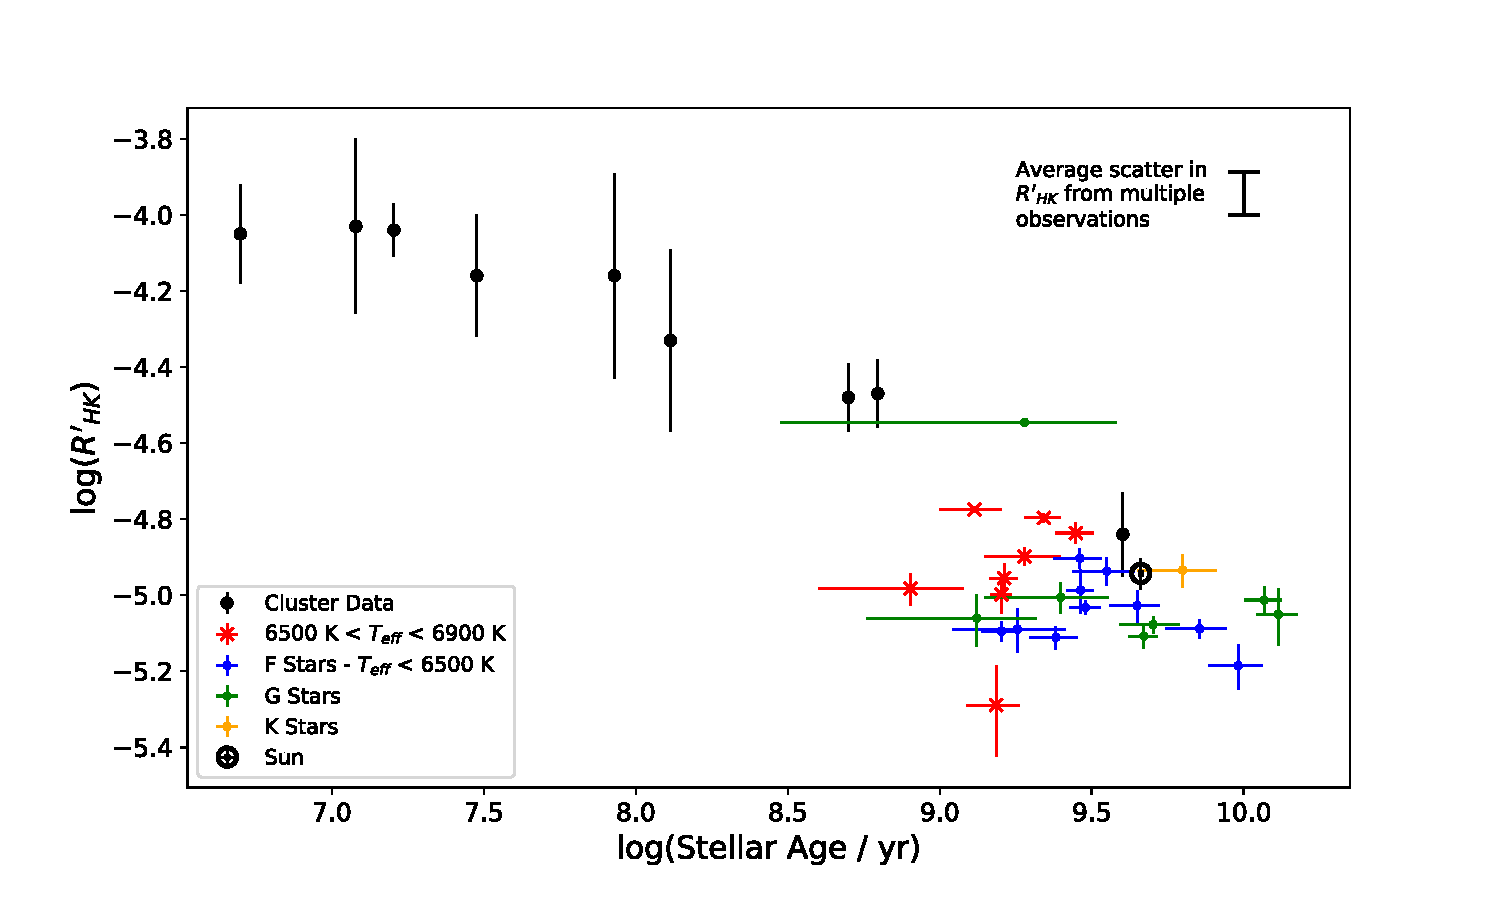
\includegraphics[width=0.99\textwidth]{Figures/4-Chromospheric_age/ca_results_with_clusters.pdf}
	\caption{Plot showing data analysed in this work alongside cluster data from \citet{Mamajek_Hillenbrand_2008} shown in black. The average solar value over several cycles is also shown \citep{Egeland_etal_2017}.}
	\centering
	\label{fig:calcium_emission_plot}
\end{figure}

The full details for each star are given in Appendix \ref{App_calcium_results}. Three stars (KIC 5774694, KIC 9139163 and KIC 10454113) had observations from both of the spectrographs considered in this work (\esp and \narval). For simplicity, only the \narval data for these stars are shown in Figure \ref{fig:calcium_emission_plot} as these have smaller associated errors in the activity measurement. 

To set the data for the old stars into context, the typical spread in chromospheric activity for a sample of young stellar clusters and M67 are shown in Figure \ref{fig:calcium_emission_plot}. This cluster data is taken from Table 6 of \citet{Mamajek_Hillenbrand_2008} with errors representative of the 68\% confidence level. \citet{Mamajek_Hillenbrand_2008} collected stellar \Rprime indicator values from the available literature in a colour range of B-V = 0.46 to 0.89, which corresponds to effective temperatures of 5000 - 6500 K and matches closely to the sample selection of K, G and mid-to-late F dwarfs considered in this work. For further comparison, the mean \Rprime value for the Sun over several cycles is also shown \citep{Egeland_etal_2017}. The age of the Sun is taken to be $4.57 \pm 0.02$ Gyr \citep{Bahcall_etal_1995}.

Figure \ref{fig:calcium_emission_plot} shows that the scatter in the \Rprime activity measurements for the old stars considered in this work is quite large. Setting the F stars with effective temperatures grater than 6500 K aside, our stars span a range of \Rprime values between $-4.5<\mathrm{log}(R^{'}_{HK})<-5.2$. One star in the sample, the G dwarf KIC 5774694, has an unusually large \Rprime value; it is also a star with a large uncertainty in its asteroseismic age. Unfortunately, only a single epoch of an activity measurement is available for this star so we cannot test if a stellar flare temporarily increased the activity of this star. Therefore, if this G dwarf is considered a potential outlier with respect to activity or age, the range of activity values displayed by the mid-F to K dwarf sample is $-4.85<\mathrm{log}(R^{'}_{HK})<-5.2$.

The activity data points for the sample of old stars considered in this work do not seem to display a strong trend with stellar age. To quantify this, Spearman's rank coefficient was calculated for the sample. The Spearman's rank coefficient ($\rho$) is a parameter-free correlation indicator and is calculated using Equation \ref{Eq:spearman_rank_coeff} where $d_{i}$ is the difference in rank between the two parameters and $n$ is the number of data points. More importantly, the Spearman's rank coefficient is independent of any specific functional form of the correlation between the two quantities. A value of 0 implies no correlation, 1 implies perfect correlation, and -1 implies perfect anticorrelation. For chromospheric activity and stellar age in the mid-F to K dwarf sample in this research, the Spearman's rank coefficient is found to the -0.038, implying that basically no correlation is present in the data.

\begin{equation}
    \rho = 1 = \frac{6\Sigma d_{i}^{2}}{n(n^{2}-1)}
    \label{Eq:spearman_rank_coeff}
\end{equation}

\subsection{Comparison with M67}
The M67 cluster has an age of $\sim 4$\,Gyr \citep{Demarque_etal_1992,VandenBerg_Stetson_2004,Bellini_etal_2010} and the chromospheric activity of ca. 70 of its member stars have been reported in the literature \citep{Giampapa_etal_2006,Mamajek_Hillenbrand_2008}. The cluster is well-studied and measurements of the stellar rotation periods make it a benchmark for the spin down of cool stars \citep{Barnes_etal_2016}. It is a useful comparison target to our old-star sample and it is displayed in Figure \ref{fig:calcium_emission_plot} as part of the \citet{Mamajek_Hillenbrand_2008} cluster data.

Surprisingly, we find that the chromospheric activity of the M67 stars is higher than what is seen in our sample of stars for similar ages. It is important to note that \citet{Mamajek_Hillenbrand_2008} calculated the \Rprime values from the measurements performed by \citet{Giampapa_etal_2006}, who studied only G-type stars in their work. So the appropriate comparison group is the old G stars in our sample, i.e. the green data points in Figure \ref{fig:calcium_emission_plot}. There the discrepancy is even more pronounced: we see that the M67 stars display an activity level roughly 0.2 dex higher than the G stars with a similar age in our sample.

Therefore, an additional analysis was performed to see if data reduction issues could be the reason for this discrepancy. To this aim, additional spectra for member stars of the three oldest clusters from \citet{Mamajek_Hillenbrand_2008}, i.e. M67, the Ursa Major (UMa) moving group and the Hyades, in the \esp and \narval archives. Unfortunately no archival observations of M67 member stars were found, however, spectra of five UMa member stars and two Hyades member stars were found. Using the two channel analysis as described in Section \ref{Chp4_data_analysis_two_channel}, the spectra were analysed to obtain the \Rprime indicator. These values for the \Rprime indicator were plotted as a function of age and compared to the \citet{Mamajek_Hillenbrand_2008} values for the cluster as shown in Figure \ref{fig:cluster_data_comparison}. 

Figure \ref{fig:cluster_data_comparison} shows that there is some scatter in the \Rprime values found from archival observations, which is to be expected given the intrinsic stellar variability of cool stars. However, there is one star that has an extremely low value for the \Rprime indicator, HD 38393. It's value for the \Rprime activity indicator is more in line with what we would expect from our old field star sample. In \citet{Mamajek_Hillenbrand_2008}, HD 38393 had measured values for the \Rprime activity indicator of $-4.77$ and $-4.82$. Upon further investigation, we found that this is classed as a double star on SIMBAD, therefore this may effect the value of the \Rprime activity indicator. With the exception of this outlier, the archival observations from \esp and \narval are in agreement with the \citet{Mamajek_Hillenbrand_2008} values. No systematic offset exists between the two data sets; therefore the difference in the activity levels between the asteroseismic sample and the cluster sample is real and discuss the possible explanations for this discrepancy in Section REF.

\begin{figure}
    \centering
    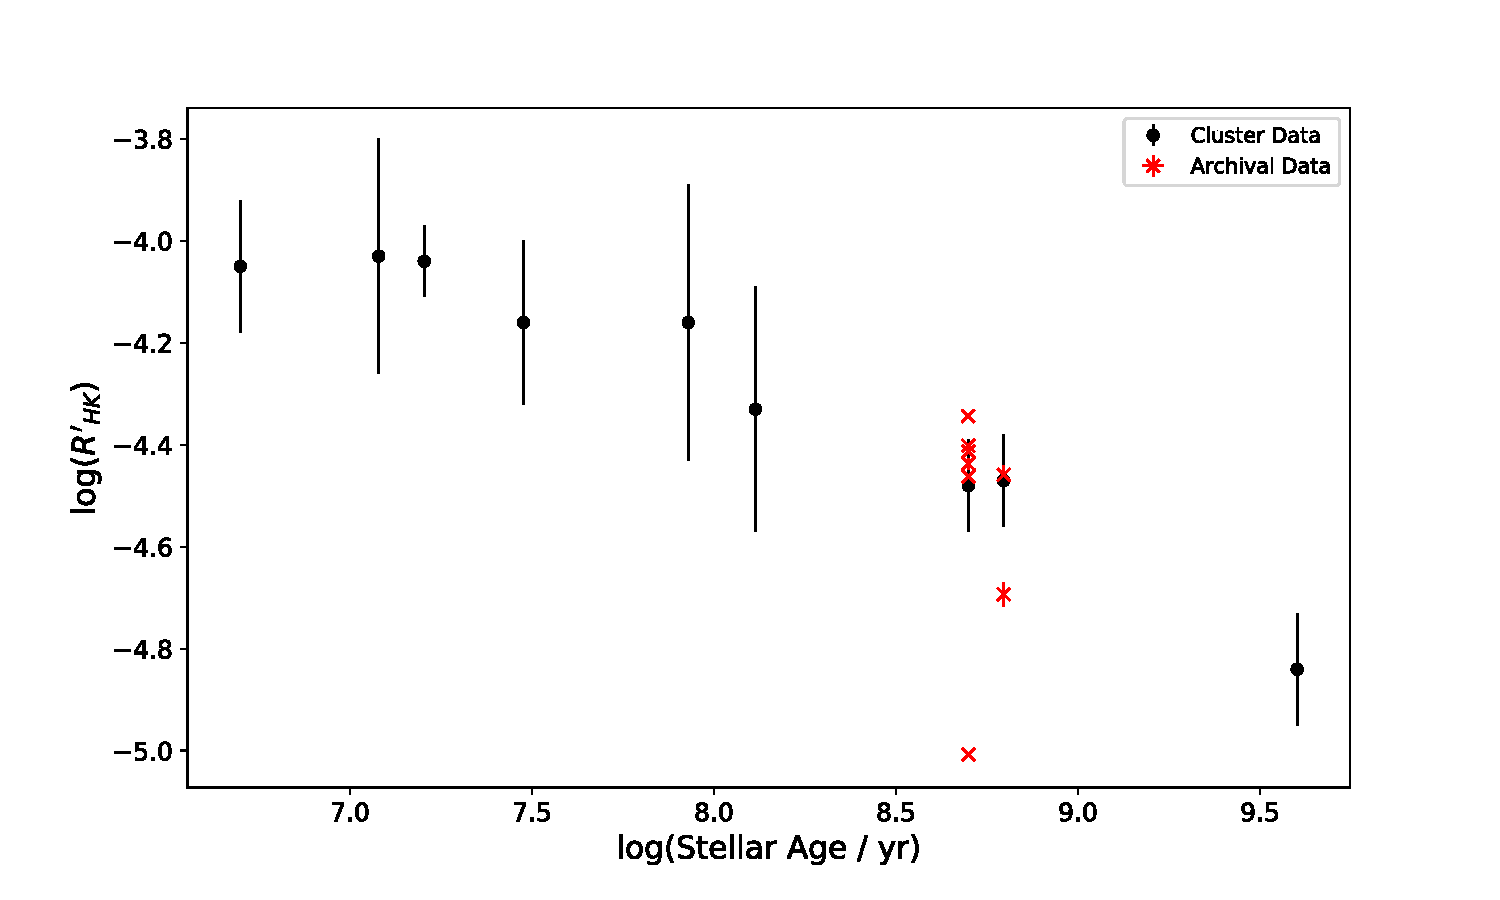
\includegraphics[scale=0.5]{Figures/4-Chromospheric_age/cluster_data.pdf}
    \caption[Analysis of cluster members]{Plot of cluster data from \citet{Mamajek_Hillenbrand_2008} alongside archival data from \esp and \narval of Ursa Major moving group and Hyades members.}
    \label{fig:cluster_data_comparison}
\end{figure}

\subsection{Variability of stars}
It is known that cool stars may have magnetic activity cycles similar to the solar eleven year activity cycle \citep{Wilson_1978,Baliunas_etal_1995}. Therefore, an investigation into the activity spread due to intrinsic stellar variability, i.e. by sample stars being in different stages of a possible activity cycle, was also conducted. The \esp and \narval archives were searched for additional observations of the sample of stars with asteroseismic ages. Thirteen of the sample stars had been observed with \esp at additional epochs. Seven of those stars are mid-F to K stars and six are hotter F stars. The details of these observations are shown in Table \ref{Table:esp_additional_obs_table}. Note that no additional observations were found in the \narval archive.

\begin{table}
\centering
\begin{tabular}{lclc}
\hline
Star Name    & Year & Product ID & Integration Time / s \\
\hline
KIC 2837475  & 2014 & 1733329i   & 145                  \\
KIC 2837475  & 2015 & 1818237i   & 78                   \\
KIC 3733735  & 2015 & 1818236i   & 70                   \\
KIC 6106415  & 2014 & 1740569i   & 60                   \\
KIC 6225718  & 2014 & 1740585i   & 60                   \\
KIC 8694723  & 2014 & 1733346i   & 255                  \\
KIC 9139151  & 2014 & 1733349i   & 280                  \\
KIC 9206432  & 2014 & 1740570i   & 250                  \\
KIC 9226926  & 2014 & 1721307i   & 210                  \\
KIC 9955598  & 2013 & 1630041i   & 1700                 \\
KIC 10454113 & 2014 & 1733354i   & 165                  \\
KIC 10454113 & 2016 & 2005115i   & 840                  \\
KIC 10709834 & 2015 & 1791287i   & 262                  \\
KIC 10963065 & 2013 & 1628074i   & 1625                 \\
KIC 11253226 & 2014 & 1740580i   & 140					\\
\hline
\end{tabular}
\caption{Details of observations taken from \esp archive to sample potential magnetic activity cycles present.}
\label{Table:esp_additional_obs_table}
\end{table}

Due to the scatter in the spectral order containing the Ca II K order in archival observations, the analysis of the chromospheric emission was conducted using the two channel method described in Section \ref{Chp4_data_analysis_two_channel}. The results of the additional observations are shown in Appendix \ref{App_ca_multiple_obs_tables}. The results of these additional observations along with the original observation for the relevant stars ($T_{eff} < 6500$ K) are shown as a function of their age in Figure \ref{fig:ca_multiple_obs}. Solar values are also shown for reference \citep{Egeland_etal_2017}. The corresponding plot for the hotter F stars is shown in Figure \ref{fig:ca_multiple_obs_hot_Fstars}. Note that the \Rprime indicator values were recalculated for the original observations using only the H and R channels for consistency, this modified activity versus age plot is shown in Appendix \ref{App_two_channel_plot}. The grey regions in Figures \ref{fig:ca_multiple_obs} and \ref{fig:ca_multiple_obs_hot_Fstars} indicated the activity region that the sample of stars occupy in the age-activity plot as determined from Figure \ref{fig:modified_ca_age_activity_plot_2channel}.

\begin{figure}
    \centering
    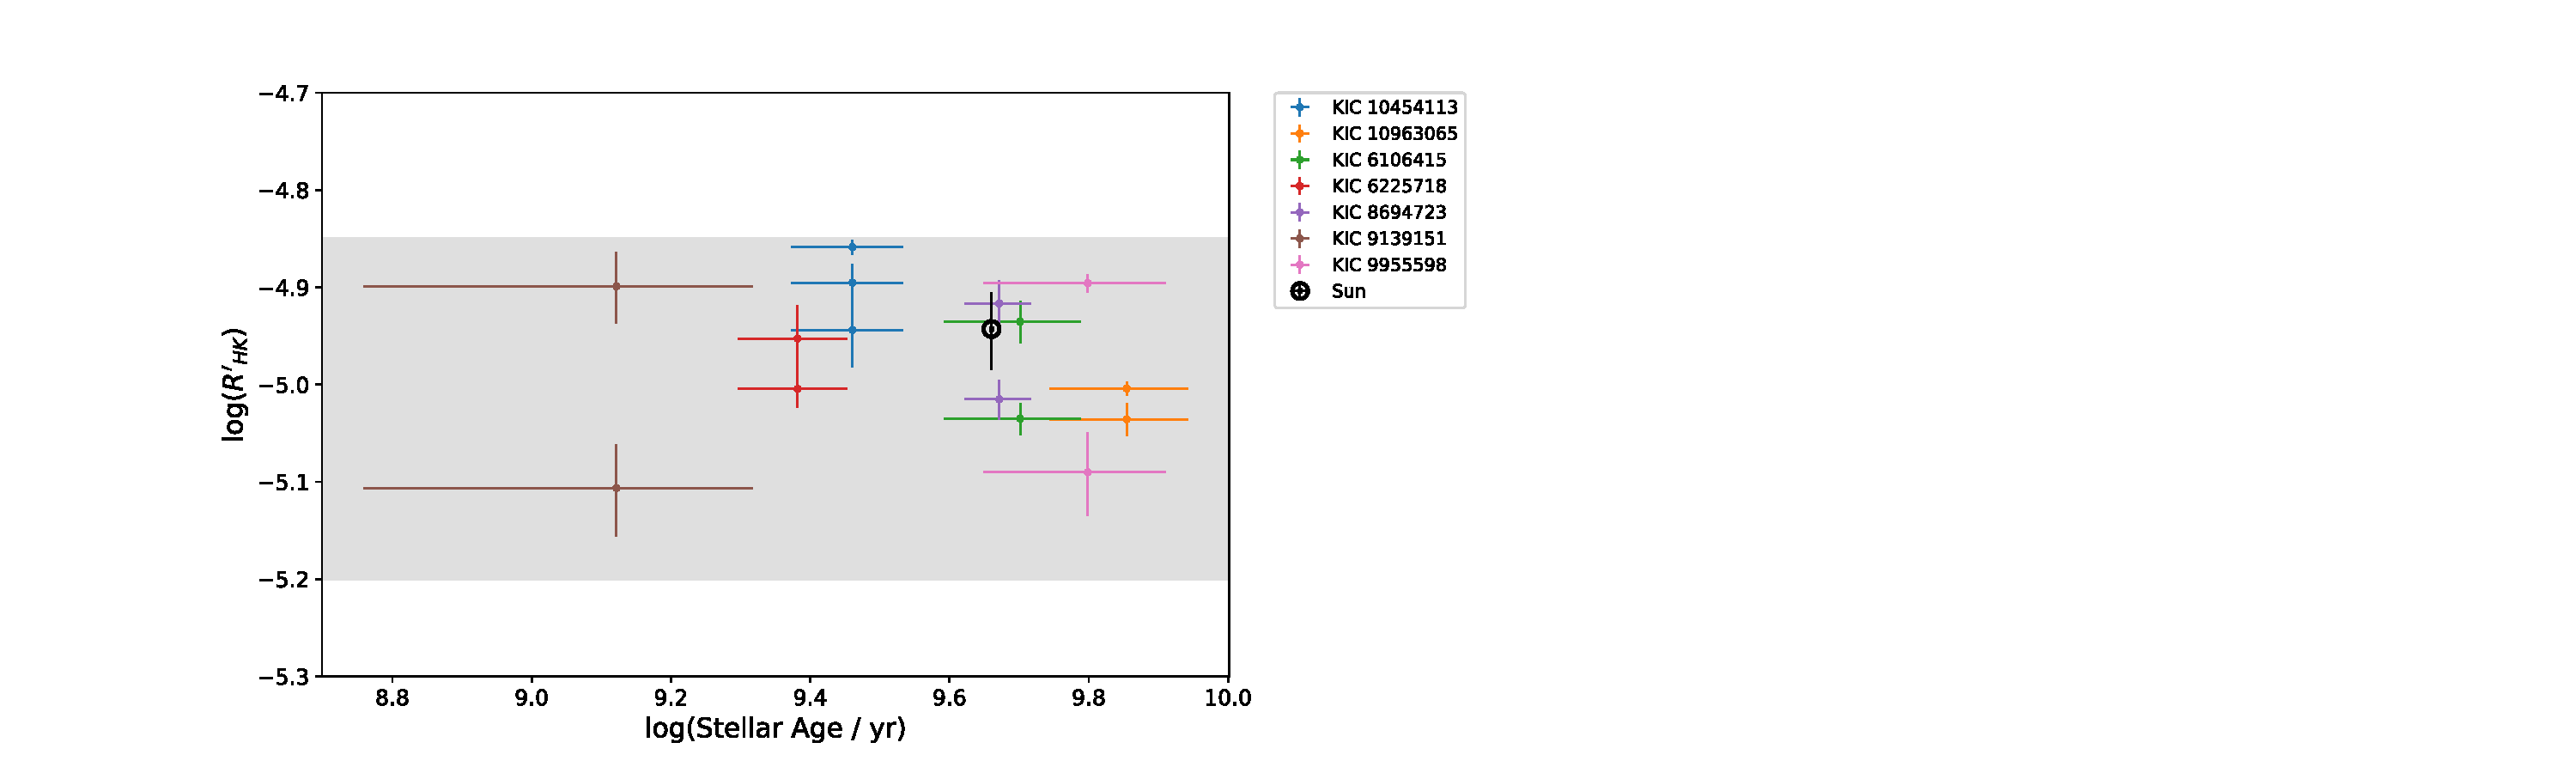
\includegraphics[scale=0.55]{Figures/4-Chromospheric_age/cool_multiple_obs_plot_with_sun.pdf}
    \caption{Plot showing the \Rprime indicator values calculated using only the H and R channels (see Section \ref{Chp4_data_analysis_two_channel} for further details) for multiple observations of stars in our sample ($T_{eff} < 6500$ K). The grey shaded region indicates the range of the \Rprime indicator values that our sample have when the \Rprime indicator is calculated using only the H and R channels (see Appendix REF for plot). The average solar value over several cycles \citep{Egeland_etal_2017} is also shown for reference.}
    \label{fig:ca_multiple_obs}
\end{figure}

\begin{figure}
    \centering
    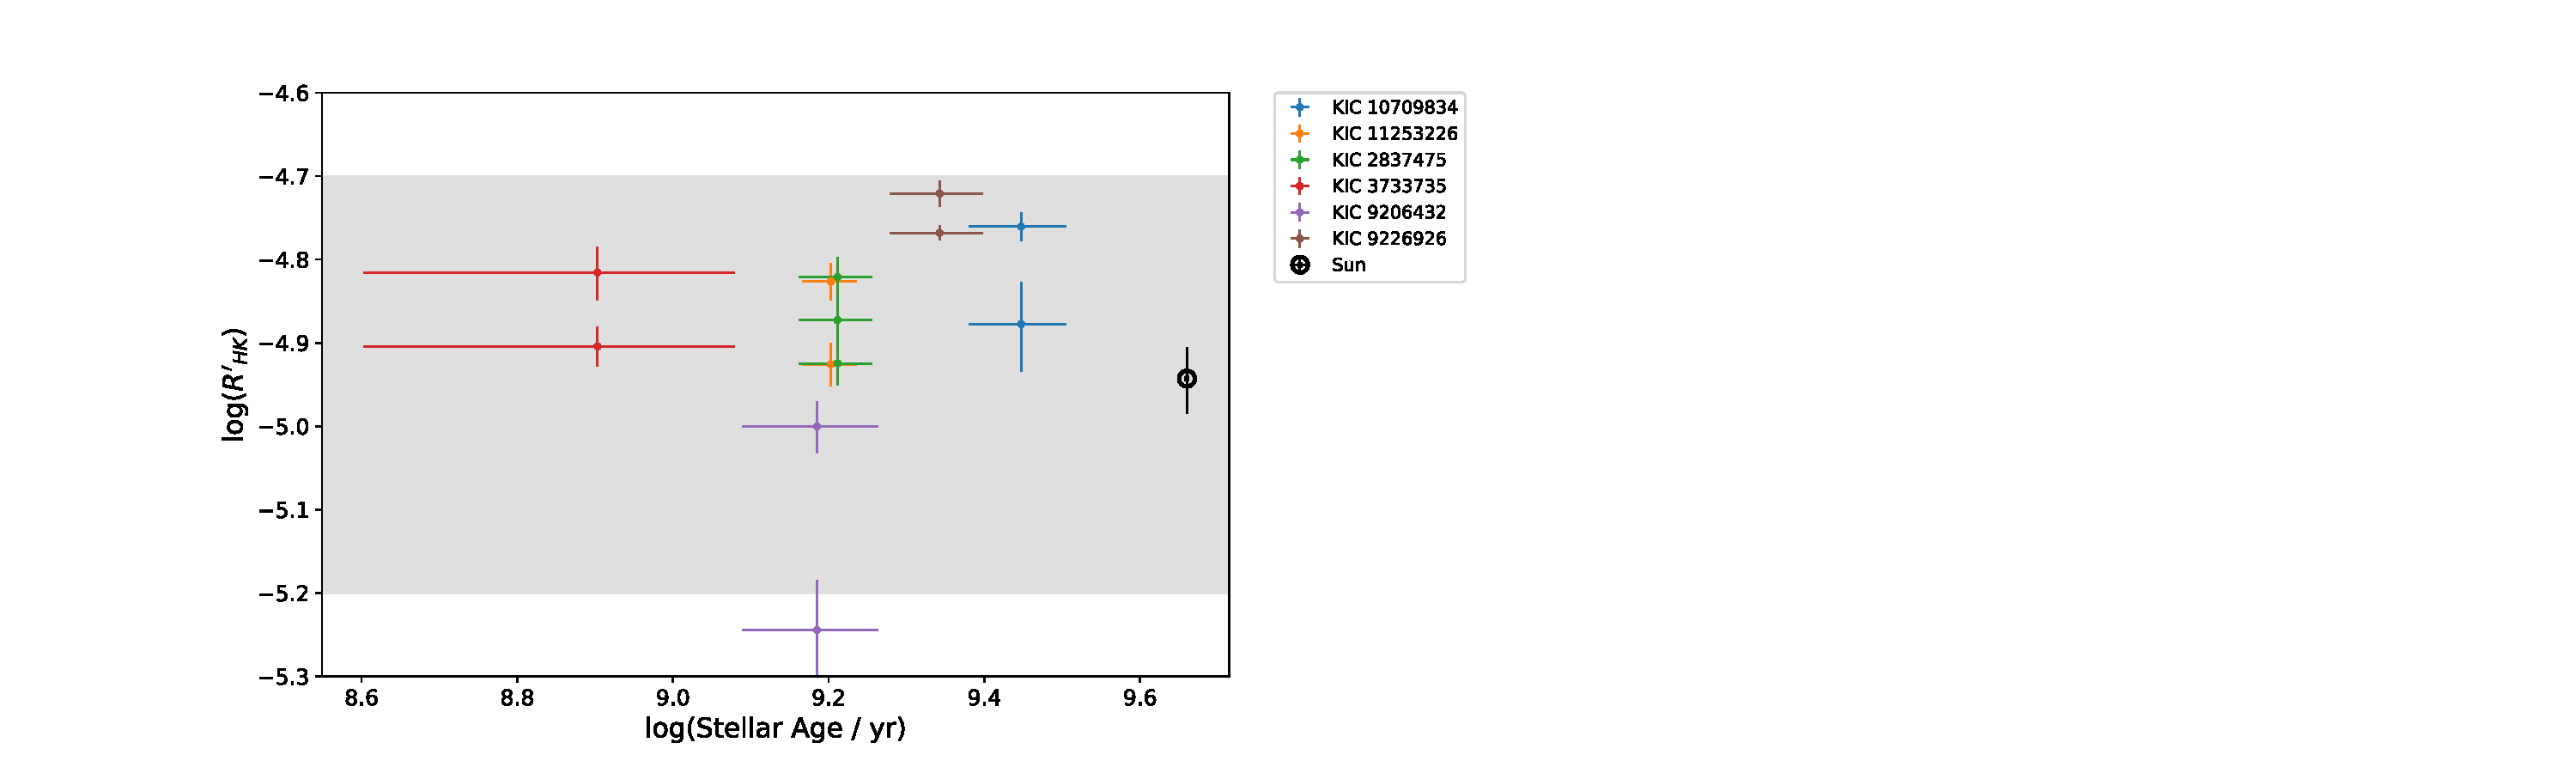
\includegraphics[scale=0.55]{Figures/4-Chromospheric_age/hot_multiple_obs_plot_with_sun.pdf}
    \caption{Plot showing \Rprime values calculated using only the H and R channels for multiple observations of stars in our sample with an effective temperature greater than 6500 K. The grey shaded region indicates the range of \Rprime values that our sample occupy.}
    \label{fig:ca_multiple_obs_hot_Fstars}
\end{figure}

\textcolor{red}{Double check the values below - I think I've calculated the correct thing!}

Firstly, considering the sample of stars with $T_{eff} < 6500$ K shown in Figure \ref{fig:ca_multiple_obs}, the plot shows that the typical intrinsic variability of individual stars with multiple observations is in the range 0.03 to 0.2 dex. The mean variability is 0.11 dex with a standard deviation of 0.062. The typical time separation of epochs is between 3 and 6 years, with the original spectra used by \citet{Bruntt_etal_2012} having been collected in 2010.

The total activity spread observed for the 17 mid-F to K stars is ca. 0.35 dex, with a mean \Rprime activity indicator of -5.033 and standard deviation of 0.076, excluding the high-activity outlier star KIC 5774694 discussed in Section \ref{Chp4_results_general_results}. This is significantly larger than the variability observed for individual stars. Therefore, the activity spread seen in Figure \ref{fig:calcium_emission_plot} is unlikely to be caused entirely by intrinsic stellar variability due to potential activity cycles.

Interestingly, the F stars with effective temperatures greater than 6500 K show similar variability properties as the cooler stars; their mean variability is 0.12 with a standard deviation of 0.061. Their variability is shown in a separate plot shown in Figure \ref{fig:ca_multiple_obs_hot_Fstars}. The total variability of the sample is larger with a spread of 0.6 dex, mainly due to one very low activity star.


\subsection{Planet-hosting stars}
From theoretical considerations \citep{Cuntz_etal_2000}, stars with exoplanets in close orbits may experience enhanced stellar activity through star-planet interaction. This effect has been observed for some systems with high-mass exoplanets (see e.g. \citealt{Poppenhaeger_Wolk_2014,Pillitteri_etal_2015}). Two of the stars in the sample have confirmed exoplanets, KIC 9955598 (Kepler-409b) and KIC 10963065 (Kepler-408b). However, Kepler-408b is a small planet with less than five Earth masses in a ca. 2.5-day orbit, and Kepler-409b has a wider orbit with ca. 69-day period \citep{Marcy_etal_2014}. Therefore it is unlikely that those two planets have a significant influence on their host stars' magnetic activity, and star-planet interactions are not expected to play a role in this investigation.

\section{Discussion}
\label{Chp4_discussion}

\subsection{Comparison to existing age-activity relationships}
There have been numerous studies that have calibrated the relationship between the \Rprime indicator and stellar age. In this section, the sample of stars with asteroseismic ages will be compared to these previous relationships.

The relationships that we consider are taken from \citet{Soderblom_etal_1991}, \citet{Lachaume_etal_1999} and \citet{Mamajek_Hillenbrand_2008}; these three relationships are shown alongside the sample of old stars analysed in this work in Figure REF

\begin{figure}
    \centering
    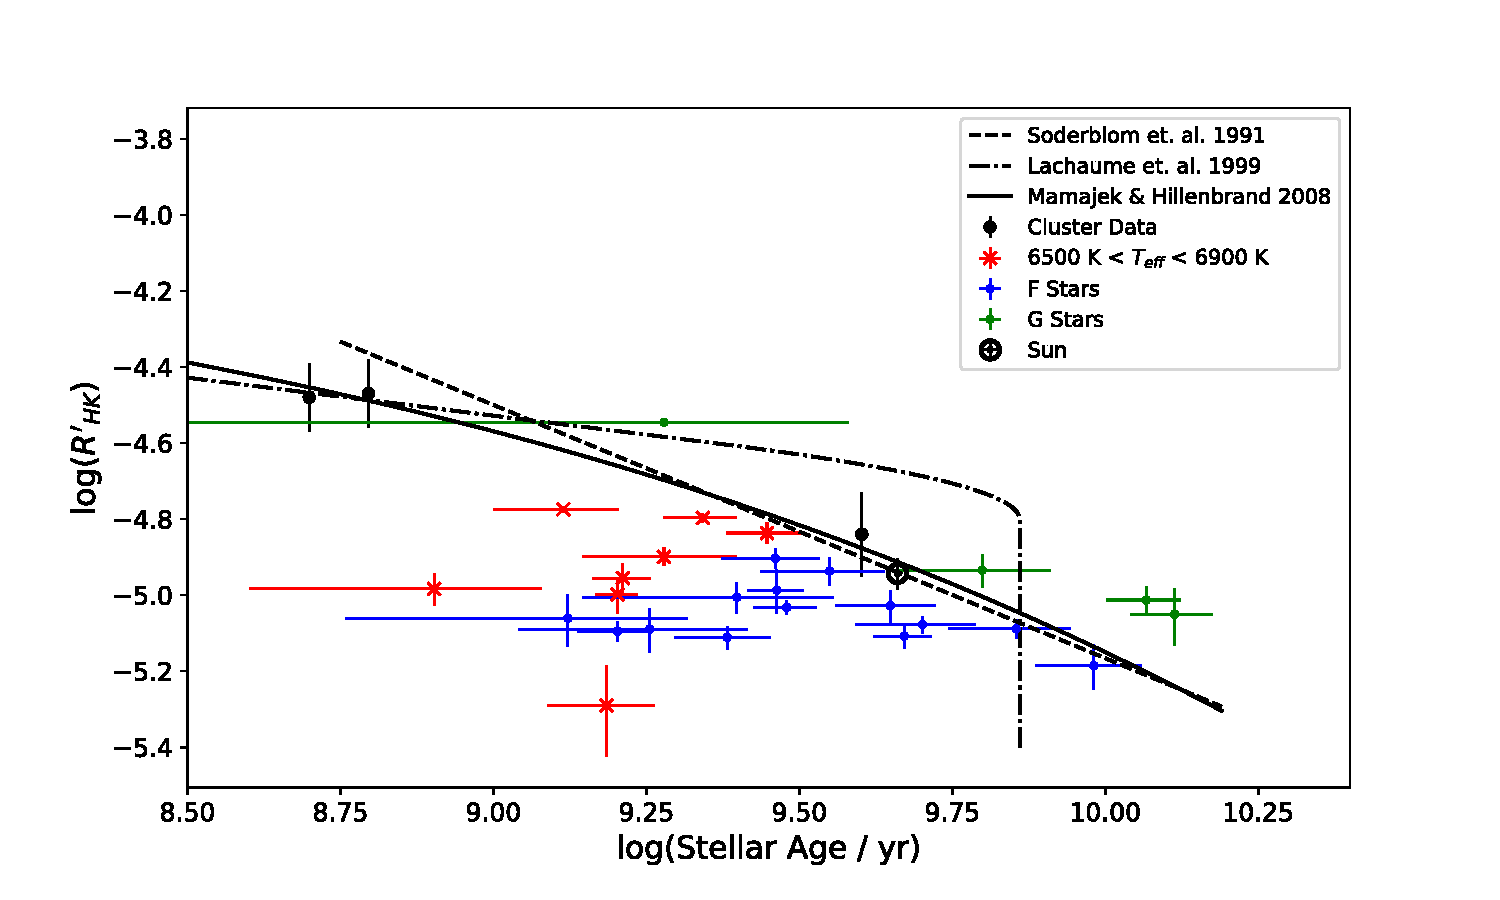
\includegraphics[scale=0.55]{Figures/4-Chromospheric_age/ca_results_3_relationship.pdf}
    \caption{Caption}
    \label{fig:comparison_previous_relationships_ca}
\end{figure}






\subsection{Spin-down in context of observational data}









\subsection{Chromospheric activity as an age indicator}









\subsection{Discrepancy between cluster stars and asteroseismic sample}








\newpage %REMEMBER TO TAKE THIS OUT!
\section{H-$\alpha$ analysis and discussion}
\label{Chp4_halpha}








\section{Conclusions}







